\documentclass[22pt]{beamer}
\usepackage[orientation=portrait, size=custom, width=91.44, height=91.44,scale=1.2]{beamerposter} % 36in*2.5 = 90cm
\usepackage[absolute,overlay]{textpos}
\usepackage{bookmark} %pdflatex says to use this to avoid errors...
\usepackage{graphicx} %for including images
\graphicspath{{figs/}} %location of images
\usepackage{wrapfig} %wrap text around the images
\usepackage{lipsum} %wrap text around the images
\usepackage{listingsutf8}    %package for code environment; use this instead of verbatim to get automatic line break; use this instead of listings to get (•)
\usepackage{amsmath}
\usepackage{gensymb}
\usepackage[export]{adjustbox}
\usepackage[skins,theorems]{tcolorbox}
\usepackage{tikz}
\newcommand*\circled[1]{\tikz[baseline=(char.base)]{
            \node[shape=circle,draw,inner sep=2pt] (char) {#1};}}
\usepackage{array}
\usepackage{booktabs,adjustbox}
\usepackage{subcaption} 

%\mode<presentation>
%this doesn't seem to make any difference; leave for now for trying out
\usetheme{Berlin}
\definecolor{MacBlue}{rgb}{0.10196,0.22353,0.53725}
\definecolor{MacMaroon} {rgb}{0.47843, 0, 0.23137}
\definecolor{MacMaroon2} {rgb}{0.47451, 0, 0}
\definecolor{MacGray}{rgb}{0.50196,0.49804,0.51765}
\definecolor{MacMaroon3}{rgb}{00.47,0.2,0.31}
\definecolor{MacGold}{rgb}{1, 0.75,0.35}
\usecolortheme[named=MacMaroon2]{structure}
\setbeamertemplate{caption}[numbered]
\setbeamertemplate{navigation symbols}{}

\title{Applying TensorFlow Machine Learning and Crowd Sourced Data to Better Understand Campus Environments: Pinpointr}
\subtitle{}  %probably want a better subtitle
  \author[Kipp, McKay, Ronald, Timpau, Deluca \& Anand]{Matthew Kipp, Sean McKay, Brandon Ronald, Victor Timpau, supervised by Dr.~Patrick Deluca and Dr.~Christopher Anand$^\dagger$ \vspace{0.3cm} \newline \small \{kippmr, mckaysm, timpauv, delucapf, anandc\}@mcmaster.ca}
  \institute[McMaster University]{$^\dagger$Department of Computing and Software, McMaster University

1280 Main St. W, Hamilton, Ontario, Canada L8S 4L8}
  \date{December 5, 2018}

\begin{document}
%compile with pdflatex

%there is only one frame, because there is only one page; yeah, it's a poster
%textblock and block seem to work nicely to organize layout
\begin{frame}[fragile]

\begin{textblock}{2}(0.7,1)

\includegraphics[height=8.5cm]{englogo.png}
\end{textblock}

\begin{textblock}{2}(12.7,0.80)

\includegraphics[height=10.5cm]{fireball-logo.png} 
\end{textblock}

\begin{textblock}{8}(4,1)
\titlepage
\end{textblock}

\begin{textblock}{7}(4.25,3.1)
\begin{figure}[htbp] %  figure placement: here, top, bottom, or page
 \centering
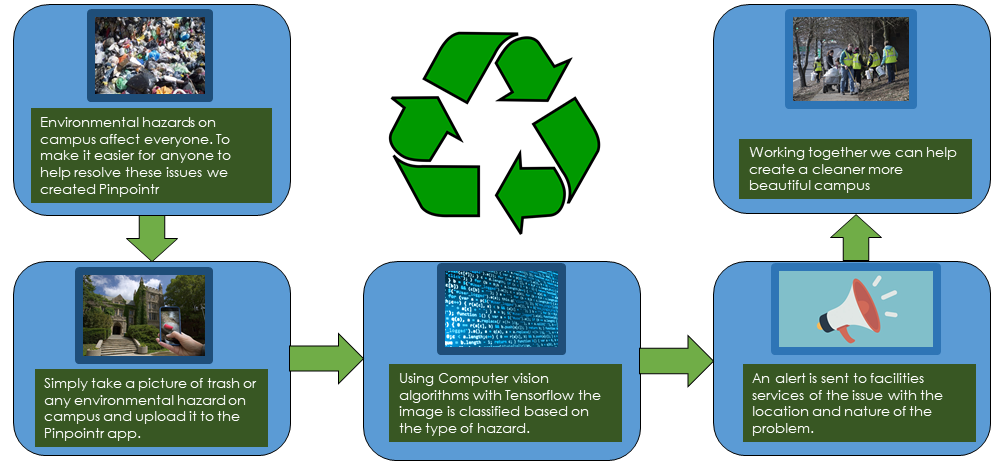
\includegraphics[height=20cm]{flowchart.png}
\end{figure}
\end{textblock}

\begin{textblock}{3.5}(0.5, 3.1)
\begin{block}{Introduction}
Over 2000 Metric tonnes of waste was generated on campus in 2017. To reduce the amount of waste disposed of improperly it’s important to have everyone on campus participate \par

Issues from full garbage cans to broken water fountains can increase the amount of waste generated. \par

To make reporting any environmental hazards or facilities issues on campus easier, we created Pinpointr, an integrated solution for managing waste on campus. 
\end{block}

\begin{block}{What is Pinpointr?}
Pinpointr is an app that allows anyone on campus to document an issue on campus with a single photo and a button press. The app uses machine learning technology and geolocation to figure out where and what the issue is. From there, it sends an alert to facilities services, so they can create a work order to deal with the issue. It also includes the ability to scan QR codes placed on facilities around campus, in order to report issues with specific trash cans, water fountains, etc.
\end{block}


%Could probably cut this down quite a bit
\begin{block}{User Adoption}
Phase 1
\begin{itemize}
\item Beta version of an app for uploading and classifying photos, locating them on a map
\item Small team of testers to determine the ease of use of the app, identify bugs on the users side
\end{itemize}
Phase 2
\begin{itemize}
\item Release revised Pinpointr app 
\item A small team of janitorial staff testing the software to see if it makes their work easier or more efficient, and identifying any existing bugs or improvements that can be made on the staff side
\end{itemize}
Phase 3
\begin{itemize}
\item Multiple platforms for sending pictures (Text, Twitter, App)
\item Greater adoption by janitorial staff
\end{itemize}
Phase 4
\begin{itemize}
\item Promotion and incentives for downloading the app and reporting environmental hazards, increasing the user base
\item Use derived metrics from the app to inform and improve purchasing decisions for other staff on campus
\end{itemize}
\end{block}

\end{textblock}

\begin{textblock}{3.5}(12, 3.1)
\begin{block}{Overall Goals}
\begin{itemize}
\item Decrease response time for dealing with environmental hazards and broken facilities
\item Provide better work metrics for custodians
\item Identify problem areas around campus, so steps can be taken to add more waste disposal options
\item Identify common sources of waste that originate on campus, so steps can be taken to reduce unnecessary packaging or transition to more environmentally friendly options
\item Reduce the amount of waste on campus by promoting awareness amongst the user base
\end{itemize}
\end{block}

\begin{block}{Conclusions \& Future Work}
\begin{figure}[htbp] %  figure placement: here, top, bottom, or page
\begin{itemize}
\item Create working AI prototype that classifies differences between different waste materials based on only a small data set.
\item Display points on map, categorize points in sections of campus or by buildings
\begin{figure}
   \centering
   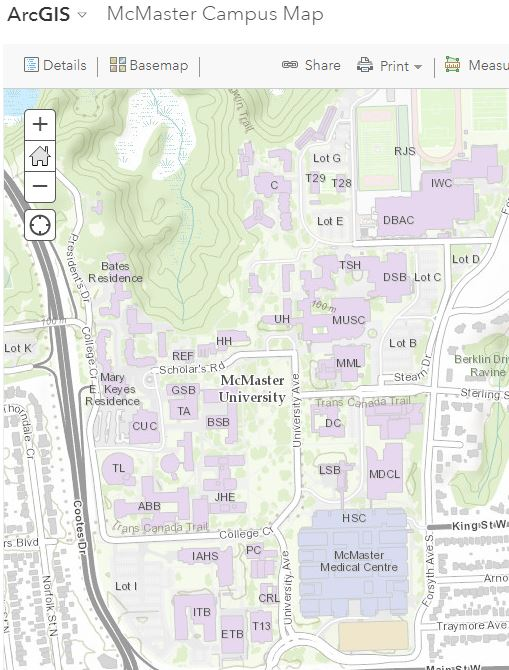
\includegraphics[height=14.5cm]{pinpointr-map.jpg}
   \label{fig:map}
\end{figure}
\item Display graduated colour charts to find hot spots around campus
\item Dynamic heatmaps based on submitted data 
\item Use ESRI and ArcGIS services and maps 
\item Leaflet.js mapping API based interface
\end{itemize}
\end{figure}
\end{block}

\begin{block}{References}
\setbeamertemplate{bibliography item}{\insertbiblabel}
\bibliographystyle{ieeetr}
{\scriptsize
\bibliography{bib}}
\end{block}

\begin{comment}
%these aren't in any particular style, it's just the basic idea
\begin{block}{References}
\setbeamertemplate{bibliography item}{\insertbiblabel}
\bibliographystyle{ieeetr}
{\scriptsize
\bibliography{bib}}
\end{block}
\vspace{-1.8mm}
%will need some more graphics to thank the various people
\end{comment}
\begin{figure}[htbp]
\centering

\includegraphics[height=5cm]{googlebrain-logo.png}
\hspace{1cm}

\includegraphics[height=5cm]{tensorflow-logo.png}
\hspace{1cm}

\includegraphics[height=5cm]{python-logo.png}
\hspace{1cm}

\includegraphics[height=5cm]{esri-logo.png}
\end{figure}

\end{textblock}

\begin{textblock}{7.25}(0.5,7.1)



\end{textblock}



\begin{textblock}{7.25}(4.375,7.1)
\begin{block}{Object Recognition with TensorFlow}
Tensor Flow
\begin{itemize}
\item Built by Google Brain, Tensorflow is an open-source combines several machine learning and deep learning models and algorithms.
\item C++ back end, Python front end.
\end{itemize}
MobileNets
\begin{itemize}
\item TFLite (“Tensorflow Lite”) models such as MobileNets provide low-latency, on-device machine learning inference requiring minimal storage space, optimal for mobile devices. 
\item MobileNets model provides a lightweight, yet powerful model with training methodology based on convolutional neural network architecture.
\end{itemize}
\begin{figure}[htbp] %  figure placement: here, top, bottom, or page
\begin{subfigure}{0.95\textwidth}
   \centering
   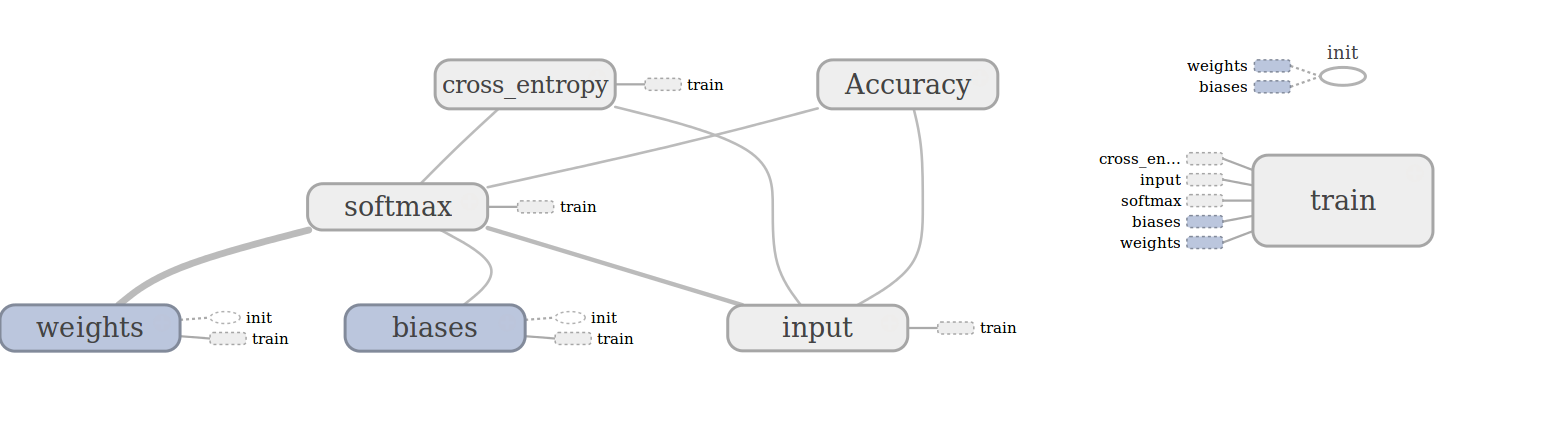
\includegraphics[height=10cm]{softmax.png}
   \caption*{\textit{Figure 1:} “softmax” represents the final output layer, providing the final object categorization and probability. The bottleneck nodes to the right represent a series of layers created during the training process.}
   \label{fig:softmax}
\end{subfigure}
\end{figure}
TensorBoard
\begin{itemize}
\item Data visualization tool for model training. Provides a platform for continuous monitoring of model accuracy. 
\end{itemize}
\begin{figure}[htbp] %  figure placement: here, top, bottom, or page
\begin{subfigure}{0.95\textwidth}
   \centering
   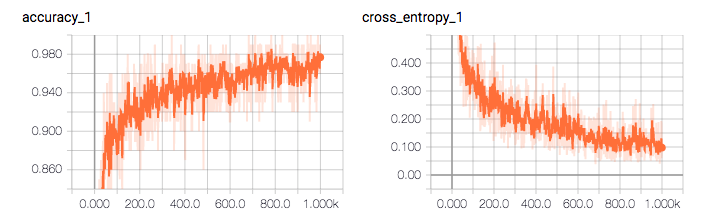
\includegraphics[height=10cm]{interface.png}
   \caption*{\textit{Figure 2:} Tensorboard Interface:  As the training dataset grows and the number of training sessions increases, the accuracy of the model approaches 1, while cross entropy approaches 0.}
   \label{fig:interface}
\end{subfigure}
\end{figure}
\end{block}
\end{textblock}


\end{frame}
\end{document}
